\documentclass[11pt]{article}
\usepackage{geometry}                % See geometry.pdf to learn the layout options. There are lots.
\geometry{letterpaper}                   % ... or a4paper or a5paper or ... 
%\usepackage[parfill]{parskip}    % Activate to begin paragraphs with an empty line rather than an indent
\usepackage{graphicx}
%\usepackage{amssymb}
\usepackage{amsmath}
\usepackage{epstopdf}
\usepackage{natbib}
\usepackage{doi}
\usepackage{tikz}
\usetikzlibrary{arrows,decorations.markings}
\bibliographystyle{plainnat}
\DeclareGraphicsRule{.tif}{png}{.png}{`convert #1 `dirname #1`/`basename #1 .tif`.png}
\newcommand{\code}[1]{\mbox{\bf#1}}

\title{Regional MOM6}
\author{Kate Hedstrom \and Alistair Adcroft \and Robert Hallberg
\and Matt Harrison \and Maria Aristizabal \and Enrique Curchitser}
\date{}                                           % Activate to display a given date or no date

\begin{document}
\maketitle
\begin{abstract}
Adding and evaluating open boundary conditions (OBCs) in MOM6.
\end{abstract}
\section{Introduction}
\section{Methods}

The goal of this project is to add open boundary conditions (OBCs)
to MOM6 such that it can be used as a regional ocean model. The open
boundaries can be placed anywhere on the model grid between $q$-points
on the Arakawa C grid, including but not limited to the boundaries of the computational domain. In fact, it is possible to create a staircase of open
boundary segments at an angle through the domain, such as seen in
Figure \ref{fdomain}. In order to support this feature, it is
necessary that nothing outside of the open boundary be used in the
model timestepping. If halo points were to be used, then both segments 2
and 3 in Figure \ref{fhalo} would be trying to set properties at
point A.

The following discussion will describe a boundary on the eastern
side of the domain, such as segment 4 in Figure \ref{fhalo}. See
Figure \ref{findices} for detailed placement on an Arakawa C grid.
Some options require a value for the boundary points; these will 
be denoted for example as $v_{\rm ext}$ for variable $v$. 

\begin{figure}
\begin{center}
\setlength{\unitlength}{10mm}
\begin{picture}(8.5,5.0)(0,0)
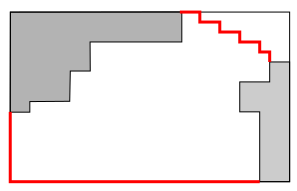
\includegraphics{pics/domain}
\end{picture}

\caption{An example of a domain with open boundary segments shown in red. Grey-shaded areas are land mask.}
\label{fdomain}
\end{center}
\end{figure}

\begin{figure}
\begin{center}
\setlength{\unitlength}{10mm}
%\begin{picture}
\begin{picture}(8,4.5)(0,0)

 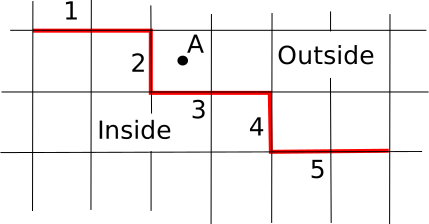
\includegraphics[width=8cm]{pics/halo}
\end{picture}
\caption{A portion of the grid with some numbered open boundary
segments. Point A is at a tracer point outside of OBC segments 2 and 3.}
\label{fhalo}
\end{center}
\end{figure}

\begin{figure}
\begin{center}
\setlength{\unitlength}{10mm}


\definecolor{cfd0000}{RGB}{253,0,0}


\begin{tikzpicture}[y=0.80pt, x=0.80pt, yscale=-1.000000, xscale=1.000000, inner sep=0pt, outer sep=0pt]
\begin{scope}[shift={(-163.5466,-431.83352)}]
  \path[draw=cfd0000,line join=miter,line cap=butt,miter limit=4.00,even odd
    rule,line width=3.200pt] (309.0437,474.0287) -- (308.5941,531.6145);
  \path[fill=black,miter limit=4.00,line width=3.200pt]
    (286.1362,503.0324)arc(0.000:89.505:5.311826 and
    4.903)arc(89.505:179.010:5.311826 and 4.903)arc(179.010:268.515:5.311826 and
    4.903)arc(268.515:358.019:5.311826 and 4.903);
  \path[draw=black,line join=miter,line cap=butt,even odd rule,line width=0.800pt]
    (164.7651,533.1417) -- (402.6996,532.0564);
  \path[draw=black,line join=miter,line cap=butt,even odd rule,line width=0.800pt]
    (163.5482,473.1356) -- (400.7699,472.3682);
  \path[draw=black,line join=miter,line cap=butt,even odd rule,line width=0.800pt]
    (250.5372,434.1369) -- (250.1654,569.4659);
  \path[draw=black,line join=miter,line cap=butt,even odd rule,line width=0.800pt]
    (369.4811,437.2064) -- (369.1094,572.5354);
  \path[draw=black,line join=miter,line cap=butt,even odd rule,line width=0.800pt]
    (308.8581,437.2064) -- (308.4863,572.5354);
  \path[draw=black,line join=miter,line cap=butt,even odd rule,line width=0.800pt]
    (189.9141,431.8347) -- (189.5424,567.1637);
  \path[fill=black,line join=miter,line cap=butt,line width=0.800pt]
    (304.3262,586.5253) node[above right] (text3379) {$i$};
  \path[fill=black,line join=miter,line cap=butt,line width=0.800pt]
    (176.4758,586.9905) node[above right] (text3383) {$i-2$};
  \path[fill=black,line join=miter,line cap=butt,line width=0.800pt]
    (236.3315,586.9905) node[above right] (text3387) {$i-1$};
  \path[fill=black,miter limit=4.00,line width=3.200pt]
    (226.2806,503.0324)arc(0.000:89.505:5.311826 and
    4.903)arc(89.505:179.010:5.311826 and 4.903)arc(179.010:268.515:5.311826 and
    4.903)arc(268.515:358.019:5.311826 and 4.903);
  \path[fill=black,line join=miter,line cap=butt,line width=0.800pt]
    (199.4973,553.2258) node[above right] (text3397) {$i-1.5$};
  \path[fill=black,line join=miter,line cap=butt,line width=0.800pt]
    (260.8877,554.7606) node[above right] (text3401) {$i-0.5$};
  \path[fill=black,line join=miter,line cap=butt,line width=0.800pt]
    (412.0616,477.2552) node[above right] (text3409) {$j$};
  \path[fill=black,line join=miter,line cap=butt,line width=0.800pt]
    (405.9225,535.5761) node[above right] (text3413) {$j-1$};
  \path[fill=black,line join=miter,line cap=butt,line width=0.800pt]
    (391.3423,506.4156) node[above right] (text3417) {$j-0.5$};
  \path[fill=black,line join=miter,line cap=butt,line width=0.800pt]
    (268.3021,517.2205) node[above right] (text3465) {$\eta$};
  \path[fill=black,line join=miter,line cap=butt,line width=0.800pt]
    (318.4652,515.7338) node[above right] (text3469) {$u$};
  \path[cm={{0.49092,-0.38205,0.38205,0.49092,(29.92447,456.97738)}},fill=black,miter
    limit=4.00,line width=0.800pt] (280.0000,382.3622) -- (277.0611,376.4073) --
    (270.4894,375.4524) -- (275.2447,370.8171) -- (274.1222,364.2720) --
    (280.0000,367.3622) -- (285.8779,364.2720) -- (284.7553,370.8171) --
    (289.5106,375.4524) -- (282.9389,376.4073) -- cycle;
  \path[cm={{0.49092,-0.38205,0.38205,0.49092,(29.92447,397.8891)}},fill=black,miter
    limit=4.00,line width=0.800pt] (280.0000,382.3622) -- (277.0611,376.4073) --
    (270.4894,375.4524) -- (275.2447,370.8171) -- (274.1222,364.2720) --
    (280.0000,367.3622) -- (285.8779,364.2720) -- (284.7553,370.8171) --
    (289.5106,375.4524) -- (282.9389,376.4073) -- cycle;
  \path[fill=black,line join=miter,line cap=butt,line width=0.800pt]
    (316.1631,466.1991) node[above right] (text3477) {$q$};
  \path[fill=black,line join=miter,line cap=butt,line width=0.800pt]
    (266.9305,463.8970) node[above right] (text3481) {$v$};
  \path[->,>=stealth,draw=black,line join=miter,line cap=butt,miter limit=4.00,even odd
    rule,line width=1.200pt] (300.0000,502.3622) -- (320.0000,502.3622);
  \path[->,>=stealth,draw=black,line join=miter,line cap=butt,miter limit=4.00,even odd
    rule,line width=1.200pt] (279.2807,482.4103) -- (279.3288,463.9932);
\end{scope}

\end{tikzpicture}



\caption{An eastern boundary segment at $i$ showing the staggered Arakawa C grid.}
\label{findices}
\end{center}
\end{figure}

\subsection{Barotropic}

\subsubsection{Specified}
For the barotropic mode, the only open boundary options are on the
velocity normal to a boundary segment. In the simplest case, one
knows both the barotropic velocity and the barotropic transport
through the OBC segments and can simply set them accordingly.
For a segment running north-south, one sets the $u$-velocity:
\begin{equation}
  \overline{u}_{i} = \overline{u}_{\rm ext}
\end{equation}
and the matching transport ($\overline{u} \, H dy$),
where $H$ is the total water depth and $dy$ is the meridional grid
spacing.

\subsubsection{Flather}

The original \citet{Flather76} algorithm is:
\begin{equation}
  \overline{u} = \overline{u}_{\rm ext} + \sqrt{\frac{g}{H}} \,
    (\eta - \eta_{\rm ext})
\end{equation}
The implementation used in MOM6 starts by finding a nondimensional
wave speed:
\begin{equation}
  C = \frac{dt}{dx} \sqrt{gH}
\end{equation}
then applying it to find an estimate of $\overline{u}$ and $\eta$ at the boundary.
If the boundary is at $i$ and we have an eastern boundary:
\begin{equation}
  u^{\star} = C \overline{u}^n_{i-1} + (1-C)\overline{u}^n_i
\end{equation}
\begin{equation}
  \eta^{\star} = \eta_{i-.5} + (0.5-C)(\eta_{i-.5} - \eta_{i-1.5})
\end{equation}
The new velocity becomes:
\begin{equation}
  \overline{u}^{n+1} = 0.5 \left( u^{\star} + \overline{u}_{\rm ext} +
    \sqrt{\frac{g}{H}} (\eta^{\star} - \eta_{\rm ext}) \right)
\end{equation}
The velocity used in the transport equation has some time filtering applied:
\begin{equation}
  \overline{u}_{\rm trans} = (1 - \beta)\overline{u}^n + \beta \overline{u}^{n+1}
\end{equation}
with $\beta > 0.05$ often set to 0.2.
[I don't know why the transport is filtered and not ubt directly.]

\subsection{Baroclinic normal velocity}
\label{sec_bc_normal}
\subsubsection{Specified}
Much like the barotropic option, one simply sets the normal flow
and the normal transport:
\begin{equation}
  u_{i} = u_{\rm ext}
\end{equation}
and the matching transport ($u \, h \, dy$),
where $h$ is the layer depth and $dy$ is the meridional grid
spacing.

\subsubsection{Gradient}
Setting the gradient to zero at the boundary requires no external values:
\begin{equation}
  u_{i} = u_{i-1}
\end{equation}

\subsubsection{Periodic}
MOM6 was designed to be used as a global model and in fact has
periodicity in the $x$-direction on by default. There is a flag to
turn it off.

\subsubsection{Radiation}
\label{S_rad}
In realistic domains, open boundary conditions can be extremely
difficult to get right. There are situations in which incoming flow and
outgoing flow happen along the same boundary or even at different
depths at the same horizontal location. \citet{Orlanski76}
proposed a radiation scheme in which a local normal phase velocity is
computed. We begin by computing a non-dimensional phase speed:
\begin{equation}
  C = \frac{u^n_{i-1} - u^{n+1}_{i-1}}{u^{n+1}_{i-1} - u^{n+1}_{i-2}}
\end{equation}
then applying limiters and a time-average to it:
\begin{align}
  C &= \max(C, 0.0) \\
  C &= \min(C, C_{\max}) \\
  C &= (1 - \gamma) * C^{n-1} + \gamma * C
\end{align}
Here, $C_{\max}$ and $\gamma$ can be set at run time, but have default
values of 10 and 0.3, respectively. The resulting phase speed is
used to update the boundary velocity:
\begin{equation}
   u_{i} = \frac{u_{i} + C * u_{i-1}}{1 + C}
\label{eqorl}
\end{equation}

\subsubsection{Oblique}
The Orlanski scheme works for a wave propagating normal to the boundary, but
has problems when waves approach the boundary at an angle.
\citet{Raymond84} have modified the scheme to account for
propagation in all three directions. In MOM6, only the two horizontal
directions are accounted for. We start by computing these terms:
\begin{align}
  C_x &= \frac{(u^n_{i-1,j} - u^{n+1}_{i-1,j})(u^{n+1}_{i-1,j} - u^{n+1}_{i-2,j})}{C_{ff}} \\
  C_{y1} &= \frac{(u^n_{i-1,j} - u^{n+1}_{i-1,j})(u^{n+1}_{i-1,j} - u^{n+1}_{i-1,j-1})}{C_{ff}} \\
  C_{y2} &= \frac{(u^n_{i-1,j} - u^{n+1}_{i-1,j})(u^{n+1}_{i-1,j+1} - u^{n+1}_{i-1,j})}{C_{ff}} \\
  C_{ff} &= (u^{n+1}_{i-1,j} - u^{n+1}_{i-2,j})^2 + (u^{n+1}_{i-1,j} - u^{n+1}_{i-1,j-1})^2 
\end{align}
Limits and time filters are also applied to these terms, as above in \ref{S_rad}.
\begin{equation}
   u_{i,j} = \frac{u_{i,j} + C_x u_{i-1,j} - C_{y1} (u_{i,j} - u_{i,j-1})}{1 + C_x}
\label{eqrka}
\end{equation}
or
\begin{equation}
   u_{i,j} = \frac{u_{i,j} + C_x u_{i-1,j} - C_{y2} (u_{i,j+1} - u_{i,j})}{1 + C_x}
\label{eqrkb}
\end{equation}
depending on the sign of $C_y$. Only the upstream component is used.

The radiation approach is appropriate for waves leaving the domain. A
check is made to see which way the phase velocity is headed. If it
is entering the domain, a zero gradient condition is applied unless
an additional nudging option is also specified as described below.

\subsubsection{Mixed radiation-nudging boundary condition}
As described in \citep{Marchesiello2001}, one has an option for
providing radiation conditions on outflow and nudging to a known
exterior value on inflow. This is implemented as a variation on the
radiation condition, requiring two timescales: the inflow nudging
timescale and the outflow nudging timescale. These timescales are
provided in the input to MOM6.

\subsection{Tangential velocity}
The tangential velocity outside of an open boundary is used in both
the horizontal viscosity and in the Coriolis terms, in both cases as
the normal gradient of the tangential velocity. There are a number of
choices for how to handle these terms. One can globally set all of
the boundary gradient terms to zero or as having no normal gradient,
independently for the Coriolis term (vorticity) and for the viscosity
term (strain).

Alternately, one can radiate or specify the boundary tangential
velocity or its gradient and then compute the boundary strain and
vorticity from this term.  The tangential velocity and its
gradient have all the same boundary options as described in
\ref{sec_bc_normal} for the normal velocity. However, the phase
speeds computed from the normal velocity are reused here to save
computational effort (the time filtering has overhead, especially
with restarts).

\subsection{Tracers}
The boundary tracers are used by the advection terms which are
computed with the PLM, PPM, or Huynh schemes (NEED REFERENCES). A
boundary can have an evolving reservoir for each tracer or a fixed
value along each boundary segment for each tracer. Two lengthscales
can be defined, one each for inflow ($L_{in}$) and outflow ($L_{out}$);
these lengthscales currently apply to all boundary segments. Here,
inflow is defined as flow from the model into the reservoir, while
outflow is flow from external data into the reservoir. We have:
$$
  u L_{in} = \max(\frac{U_{flux} }{L_{in} dz dy}, 0.0)
$$
$$
  u L_{out} = \min(\frac{U_{flux} }{L_{out} dz dy}, 0.0)
$$
\begin{equation}
  T_{res} = \frac{ T_{res} + dt (u L_{in} T_{in} - u L_{out} T_{out})}
  {1 + dt (u L_{in} - u L_{out})}
\end{equation}
where $U_{flux}$ is the volume flux through a face of area $dz dy$,
$T_{res}$ is the tracer value in the reservoir, $T_{in}$ is the
tracer value at the interior point adjacent to the boundary, and
$T_{out}$ is the tracer value from external data for that boundary.

[WHAT ABOUT TRACER DIFFUSION AT BOUNDARIES??]

\subsection{Masking}
It is required that any region outside of the open boundary segments
be masked as land and that no computations will be done there, such
as in the NE corner in Figure \ref{fdomain}. Also, if there are
masked points along an open boundary segment, the model will handle
it appropriately. Thus, many domains can simply have four open
boundary segments, one on each side, with masking of any land bits
that should happen to cross these segments.

For domains with analytic grids, the easiest way to mask the outside
areas is to ask the model to mask it for you, using the MASK\_OUTSIDE\_OBCS
flag. It will check this in two ways and complain if it finds an
inconsistency in the resulting land mask. Check the rotated\_seamount/faulty
case for an example.

\section{Test problems}
\subsection{Barotropic Kelvin wave}
\subsection{Tracers}
\section{A realistic problem}
\section{Conclusions}
\section{Discussion}

\section{Equations of motion}

\begin{alignat}{2}
\rho_0 \left( \frac{\partial \mathbf{u}}{\partial t} + \frac{( f + \zeta )}{h} \, \hat{\mathbf{z}} \wedge h \, \mathbf{u} + { \color{red} \dot{r} \, \frac{\partial \mathbf{u}}{\partial r} } + \nabla_r K \right) &= -\nabla_r \, p - \rho \nabla_r \, \Phi + \nabla_r \cdot \boldsymbol{\mathcal{F}}
&\mbox{momentum} \label{eq:h-horz-momentum} \\
\rho \, \delta_r \Phi + \delta_r p &= 0
&\mbox{hydrostatic} \label{eq:h-hydrostatic-equation} \\
\frac{\partial h}{\partial t} + \nabla_r \cdot \left( h \, \mathbf{u} \right) + {\color{red} \delta_r ( z_r \dot{r} ) } &= 0
&\mbox{thickness} \label{eq:h-thickness-equation} \\
\frac{\partial ( \theta \, h )}{\partial t} + \nabla_r \cdot \left( \theta h \, \mathbf{u} \right) + {\color{red} \delta_r ( \theta \, z_r \dot{r} ) } &=  h \boldsymbol{\mathcal{N}}_\theta^\gamma - \delta_r J_\theta^{(z)}
&\mbox{potential temp} \label{eq:h-temperature-equation} \\
\frac{\partial ( S \, h )}{\partial t} + \nabla_r \cdot \left( S \, h \, \mathbf{u} \right) + {\color{red} \delta_r ( S \, z_r \dot{r} ) } &= h \boldsymbol{\mathcal{N}}_S^\gamma - \delta_r J_S^{(z)}
&\mbox{salinity} \label{eq:h-salinity-equation} \\
\rho &= \rho\left( S, \theta, -g \rho_0 z(r) \right)
&\mbox{equation of state,}
\label{eq:h-equation-of-state}
\end{alignat}

The primary finite volume cells are labelled with half-integers, i.e. $i \in \{\frac{1}{2},\frac{3}{2},\ldots,N_i-\frac{1}{2}\}$, The equations solved in these cells are:
$j \in \{\frac{1}{2},\frac{3}{2},\ldots,N_j-\frac{1}{2}\}$:
\begin{align}
\rho \, \delta_r \Phi + \delta_r p &= 0
\\
\frac{\partial h}{\partial t} + \delta_x U + \delta_y V &= 0
\\
\frac{\partial ( \theta \, h )}{\partial t} + \delta_x \left( \overline{\theta}^i U \right) + \delta_y \left( \overline{\theta}^j V \right) &=  h \boldsymbol{\mathcal{N}}_\theta^\gamma - \delta_k J_\theta^{(z)}
\\
\frac{\partial ( S \, h )}{\partial t} + \delta_x \left( \overline{S}^i U \right) + \delta_y \left( \overline{S}^j V \right) &= h \boldsymbol{\mathcal{N}}_S^\gamma - \delta_k J_S^{(z)}
\end{align}
The quantities $U$ and $V$ are thickness fluxes which must be identically evaluated in the continuity and tracer equations for consistency. They are notionally discretized as $U=\overline{h}^iu$ and $V=\overline{h}^jv$ but where the $h$ in these expressions is not a simple interpolation ($^{\overline{\,\,\,}i}$) but an upstream average and calculated with a positive definite reconstruction or flux limiter. In the primary cell equations, the horizontal fluxes naturally fall on the cell edges and thus require boundary conditions on open boundaries. Similarly the $\overline{S}^i$ in $\overline{S}^iU$ is upstreamed and might be flux limited in some way. The specification of the normal thickness flux at open boundaries will be mentioned below. The specification of the scalar being transported, whether $h$, $\theta$ or $S$, is usually flow dependent. For outward flow, upstreaming involves boundary values only through the reconstruction scheme. For inward flow, the scalar values are usually specified and not a function of the interior state.

The i-direction momentum equation for component $u$ is solved on the edge with integer $i$ and half-integer $j$ labels, i.e. $i \in \{0,1,\ldots,N_i\}$, $j \in \{\frac{1}{2},\frac{3}{2},\ldots,N_j-\frac{1}{2}\}$:
\begin{align}
\rho_0 \left( \frac{\partial u}{\partial t}
- \overline{ q \overline{V}^i }^j + \delta_x K \right)
&= - \delta_x p - \rho \delta_x \Phi
+ \delta_x {F}^{(xx)}  + \delta_y {F}^{(xy)} + \partial_r {F}^{(xz)}
\end{align}

The j-direction momentum equations for component $v$ is solved on the edge with $i \in \{\frac{1}{2},\frac{3}{2},\ldots,N_i-\frac{1}{2}\}$, $j \in \{0,1,\ldots,N_j\}$:
\begin{align}
\rho_0 \left( \frac{\partial v}{\partial t}
+ \overline{ q \overline{U}^j }^i + \delta_y K \right)
&= -\delta_y p - \rho \delta_y \Phi
+ \delta_x {F}^{(xy)}  + \delta_y {F}^{(yy)} + \partial_r {F}^{(yz)}
\end{align}

At open boundaries, the momentum equation for the normal flow is replaced by a new equation for the normal flow, rather than discretizing the momentum equation on the boundary.

\bibliography{ocean}
\end{document}  

